\documentclass[a4paper, 12pt]{article}

\input{"$HOME/Desktop/Studia/LaTeX/setup.tex"}

\usepackage{svg}

\title{\textsc{Monte Carlo: całkowanie metodą warstwową}\\ - sprawozdanie}
\author{Wojciech Orłowski}
\date{\today}

\begin{document}
    \maketitle

    \section{Wstęp}
    
    W ćwiczeniu zostaną obliczone całki oznaczone korzystając z bardziej zaawansowanych metod Monte Carlo (MC).
    Poza najprostszym całkowaniem MC, tutaj nazywanym metodą podstawową, zostanie zaimplementowana także metoda losowania warstwowego.
    Losowanie warstwowe możemy przeprowadzać na dwa sposoby - bez uwzględniania kształtu funkcji (metoda losowania systematycznego) oraz z uwzględnianiem kształtu funkcji całkowanej (metoda losowania warstwowego).
    Trzy całki, które należy obliczyć to:
    \begin{gather}
        C_1 = \int_{-3}^{3} \dd x \left( 1 + \tanh(x) \right), \\ 
        C_2 = \int_{0}^{10} \dd x \left( \frac{1}{1+x^2} \right), \\ 
        C_3 = \int_{0}^{1} \dd x \cos^{10}(\pi x).
    \end{gather}

    
    \subsection*{Metoda podstawowa} 

    W metodzie podstawowej losowana jest liczba $x_i$ z rozkładu jednorodnego na przedziale $(a,b)$:
    \begin{equation}
        x_i = a + (b-a)\cdot U_i; \; \; \;  U_i \sim U(0,1),
    \end{equation}
    a następnie przybliżamy wartość całki średnią z próby:
    \begin{equation}
        C = \int_{a}^{b} \dd x f(x) \approx \frac{1}{N} \sum_{i=1}^{N} (b-a)\cdot g(x_i), \;\;\;\; x_i \sim U(a,b).
    \end{equation}
    W metodzie tej nie kontrolujemy w żaden sposób ilości wylosowanych próbek w podprzedziałach.
    Dla każdej z całek losowania będą takie same.

    \subsection*{Metoda systematycznego losowania}

    W tej metodzie dzielimy odcinek $(a,b)$ na $M$ równych podprzedziałów.
    Następnie w każdym z podprzedziałów losowana jest równa ilość punktów o rozkładzie jednorodnym.
    Jeżeli chcemy, aby całkowita ilość punktów była taka sama, jak w metodzie podstawowej, w każdym podprzedziale musimy wylosować $N_m = N/M$ punktów.
    Następnie w każdym z podprzedziałów liczymy pierwszy i drugi moment zwykły
    \begin{equation}
        \bar{g^n}_m = \frac{1}{N_m} \sum_{i=1}^{N_m} \left[ (b-a) \cdot g(x_{mi}) \right]^n,
    \end{equation}
    gdzie $n = 1,2$, a $x_{mi}$ oznacza $i$-tą liczbę wylosowaną w $m$-tym podprzedziale.
    Wartość całki szacujemy jako wartość średnią pierwszych momentów
    \begin{equation}
        C \approx \sum_{m=1}^{M} \frac{N_m}{N} \bar{g^1}_m.
    \end{equation}  
    Wariancję szacujemy jako 
    \begin{equation}
        \sigma_g^2 = \sum_{m = 1}^{M} \frac{N_m}{N^2} \sigma^2_m,
    \end{equation}
    gdzie $\sigma_m^2$ to wariancja w $m$-tym podprzedziale obliczona jako
    \begin{equation}
        \sigma^2_m = \bar{g^2}_m - \bar{g_m}^2. 
    \end{equation}

    \subsection*{Optymalna metoda losowania warstwowego}

    Metoda ta analogiczna do losowania systematycznego, jednak ilość losowań w każdym podprzedziale jest różna.
    Liczba losowań jest najpierw oszacowana za pomocą metody podstawowej. 
    W podprzedziałach o większej oszacowanej wariancji zostanie wylosowana większa liczba próbek zgodnie z wzorem
    \begin{equation}
        N_m  = \frac{\hat{\sigma_m}}{\sum_{i = 1}^{M} \hat{\sigma_i}}N,
    \end{equation}
    gdzie $\hat{\sigma_i}$ oznacza odchylenie standardowe (pierwiastek z wariancji) w $i$-tym podprzedziale.
    Warto jednak zwrócić uwagę na charakter tych liczb.
    Całkowita liczba wylosowanych próbek w tym przypadku może nie być równa $N$ ze względu na błędy zaokrągleń.
    Dla dużej ilości próbek nie powinno to mieć jednak znaczenia.

    \section{Wyniki}

    Wyniki dla przeprowadzonych losowań dla każdej z całek zostały zebrane w postaci liczbowej.
    Dla optymalnej metody losowania warstwowego ilość losowań w podprzedziale estymowana była za pomocą metody podstawowej, gdzie ilość próbek losowanych do oszacowania wynosiosła 100, gdy $N = 100$, oraz 1000, gdy $N > 100$.
    Dla każdej z metod wykonano obliczenia dla $N = 10^k, \; \; k = 2,3,4,5$.
    Wyniki przedstawiono poniżej.

\begin{verbatim}
        N = 100; f(x) = 1 + tanh(x); Dokładna wartość = 6.0
        Metoda podstawowa   :  C = 6.28233 ;std-dev = 0.48036;
        Metoda systematycza :  C = 5.99694 ;std-dev = 0.04520;
        Metoda warstwowa    :  C = 5.99622 ;std-dev = 0.03309;
        
        N = 1000; f(x) = 1 + tanh(x); Dokładna wartość = 6.0
        Metoda podstawowa   :  C = 6.38258 ;std-dev = 0.15416;
        Metoda systematycza :  C = 6.00890 ;std-dev = 0.01525;
        Metoda warstwowa    :  C = 6.00648 ;std-dev = 0.01124;
        
        N = 10000; f(x) = 1 + tanh(x); Dokładna wartość = 6.0
        Metoda podstawowa   :  C = 5.96828 ;std-dev = 0.04909;
        Metoda systematycza :  C = 6.00268 ;std-dev = 0.00493;
        Metoda warstwowa    :  C = 5.99356 ;std-dev = 0.00346;
        
        N = 100000; f(x) = 1 + tanh(x); Dokładna wartość = 6.0
        Metoda podstawowa   :  C = 6.01632 ;std-dev = 0.01553;
        Metoda systematycza :  C = 6.00232 ;std-dev = 0.00154;
        Metoda warstwowa    :  C = 6.00088 ;std-dev = 0.00109;
        
        N = 100; f(x) = 1 / (1 + x^2); Dokładna wartość = 1.47113
        Metoda podstawowa   :  C = 1.76010 ;std-dev = 0.29007;
        Metoda systematycza :  C = 1.44186 ;std-dev = 0.05372;
        Metoda warstwowa    :  C = 1.41753 ;std-dev = 0.02877;
        
        N = 1000; f(x) = 1 / (1 + x^2); Dokładna wartość = 1.47113
        Metoda podstawowa   :  C = 1.52085 ;std-dev = 0.07863;
        Metoda systematycza :  C = 1.45094 ;std-dev = 0.01765;
        Metoda warstwowa    :  C = 1.48864 ;std-dev = 0.00960;
        
        N = 10000; f(x) = 1 / (1 + x^2); Dokładna wartość = 1.47113
        Metoda podstawowa   :  C = 1.48730 ;std-dev = 0.02382;
        Metoda systematycza :  C = 1.48161 ;std-dev = 0.00586;
        Metoda warstwowa    :  C = 1.47056 ;std-dev = 0.00303;
        
        N = 100000; f(x) = 1 / (1 + x^2); Dokładna wartość = 1.47113
        Metoda podstawowa   :  C = 1.47283 ;std-dev = 0.00754;
        Metoda systematycza :  C = 1.47323 ;std-dev = 0.00185;
        Metoda warstwowa    :  C = 1.47378 ;std-dev = 0.00095;
        
        N = 100; f(x) = cos(pi x)^10; Dokładna wartość = 0.24609375
        Metoda podstawowa   :  C = 0.22131 ;std-dev = 0.03187;
        Metoda systematycza :  C = 0.24681 ;std-dev = 0.00916;
        Metoda warstwowa    :  C = 0.24664 ;std-dev = 0.00566;
        
        N = 1000; f(x) = cos(pi x)^10; Dokładna wartość = 0.24609375
        Metoda podstawowa   :  C = 0.23651 ;std-dev = 0.01081;
        Metoda systematycza :  C = 0.24776 ;std-dev = 0.00263;
        Metoda warstwowa    :  C = 0.24664 ;std-dev = 0.00190;
        
        N = 10000; f(x) = cos(pi x)^10; Dokładna wartość = 0.24609375
        Metoda podstawowa   :  C = 0.24312 ;std-dev = 0.00337;
        Metoda systematycza :  C = 0.24543 ;std-dev = 0.00085;
        Metoda warstwowa    :  C = 0.24593 ;std-dev = 0.00059;
        
        N = 100000; f(x) = cos(pi x)^10; Dokładna wartość = 0.24609375
        Metoda podstawowa   :  C = 0.24644 ;std-dev = 0.00108;
        Metoda systematycza :  C = 0.24590 ;std-dev = 0.00027;
        Metoda warstwowa    :  C = 0.24561 ;std-dev = 0.00019;
\end{verbatim}           

\noaka Analizując powyższe wyniki można stwierdzić, że metoda losowania systematycznego generuje mniejsze błędy niż metoda podstawowa, a metoda losowania warstwowego mniejsze niż metoda losowania systematycznego.
Wynika to między innymi z wartości odchyleń standardowych, oznaczonych jako std-dev, a liczonych jako pierwiastek z wariancji.
Są one najmniejsze dla metody warstwowej (optymalnej).
Jednak wartość całki nie zawsze jest bliższa wartości dokładnej, jak przykładowo w przypadku wartości całki z $f(x) = \cos(\pi x)^{10}$ dla 10000 losowań, gdzie dokładniejszy wynik uzyskano metodą systematyczną.
Wynika to oczywiście z przypadku, który rządzi w wszystkich metodach Monte Carlo, taki wynik został uzyskany tylko dla jednego losowania.
Jednak wartość odchylenia standardowego czy wariancji określa przedział ufności według testów statystycznych, dlatego warto dokładność mierzyć tym parametrem.
\\
\\
Dla każdej z funkcji zostały także zebrane histogramy ilości wylosowanych próbek w każdym z przedziałów.
Zostały one przedstawione na rys. \ref{fig:histogramy}.
\begin{figure}[H]
    \centering
    \begin{subfigure}{0.49\textwidth}
        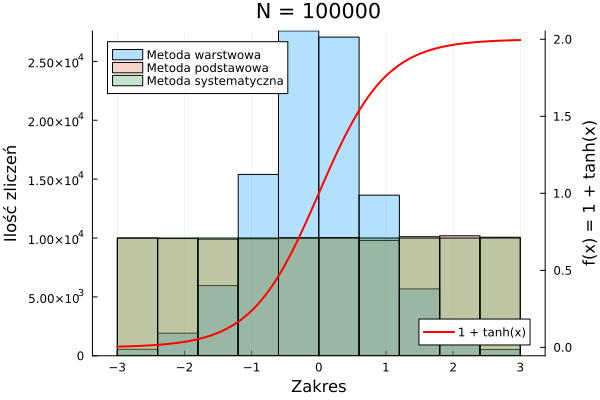
\includegraphics[width=\textwidth]{../gallery/f1.png}
        \caption{}
    \end{subfigure}
    \begin{subfigure}{0.49\textwidth}
        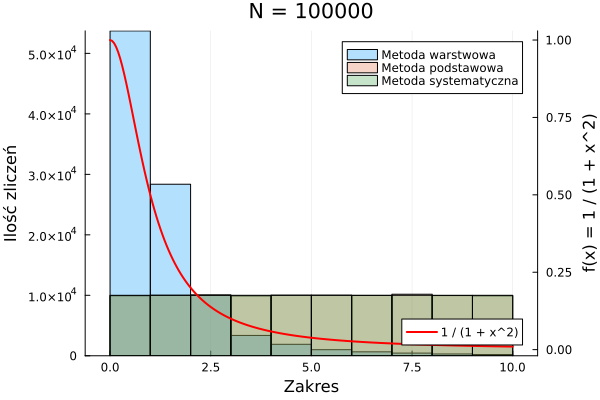
\includegraphics[width=\textwidth]{../gallery/f2.png}
        \caption{}
    \end{subfigure}
    \begin{subfigure}{0.49\textwidth}
        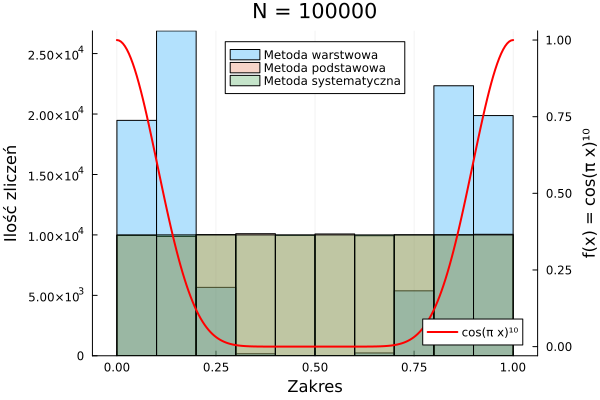
\includegraphics[width=\textwidth]{../gallery/f3.png}
        \caption{}
    \end{subfigure}
    \caption{Histogramy ilości wylosowanych próbek (N=10000) w przedziałach dla (a) pierwszej całki $C_1$, (b) drugiej całki $C_2$, (c) trzeciej całki $C_3$.}
    \label{fig:histogramy}
\end{figure}

\noaka Dla metody podstawowej ilość losowań jest podobna w każdym z podprzedziałow, ale ostatecznie różna. 
W metodzie losowania systematycznego ilość losowań jest dokładnie taka sama.
Dla dużej ilości próbek nie widać różnicy w ilości rysowań na histogramie między metodą losowania systematycznego a metodą podstawową.
Dla małej ilości próbek ($N=100$) różnice są widoczne, a analogiczne histogramy zostały przedstawione na rys. \ref{fig:hist_2}.
\begin{figure}[H]
    \centering
    \begin{subfigure}{0.49\textwidth}
        \includegraphics[width=\textwidth]{../gallery/f1_low.png}
        \caption{}
    \end{subfigure}
    \begin{subfigure}{0.49\textwidth}
        \includegraphics[width=\textwidth]{../gallery/f2_low.png}
        \caption{}
    \end{subfigure}
    \begin{subfigure}{0.49\textwidth}
        \includegraphics[width=\textwidth]{../gallery/f3_low.png}
        \caption{}
    \end{subfigure}
    \caption{Histogramy ilości wylosowanych próbek (N=100) w przedziałach dla (a) pierwszej całki $C_1$, (b) drugiej całki $C_2$, (c) trzeciej całki $C_3$.}
    \label{fig:hist_2}
\end{figure}

\noaka Największe różnice w ilości wylosowanych próbek w każdym z podprzedziałów są widoczne w metodzie losowania warstwowego.
Duża ilość wylosowanych próbek w podprzedziale występuje wtedy, gdy w danym podprzedziale jest duża zmiana wartości funkcji.
Dla funkcji o dużej zmienności ciężko jest oszacować wartość całki, dlatego w takich przedziałach stosuje się większą liczbę losowań.
Ciekawym jest fakt, że nawet 100 losowań potrzebnych do estymacji odchylenia jest wystarczające aby dobrze wyznaczyć ilość losowań w podprzedziale (rys. \ref{fig:hist_2}.)

\section{Podsumowanie}

W ćwiczeniu udało się zaaplikować bardziej zaawansowane algorytmy obliczania całek metodą Monte Carlo.
Zostało to wykonane niewielkim kosztem obliczeniowym, bo wymagało to tylko początkowej estymacji ilości losowań w podprzedziałach.
Zysk z wykonania takich operacji był wysoki, gdyż wartości odchylenia standardowego zostały skutecznie obniżone w każdym z przypadków.
Całki zostały obliczone z wysoką dokładnością, bo dla największej ilości losowań przy metodzie warstowej wyniki były zgodne do 2 miejsc po przecinku.
W ćwiczeniu zastosowana największa ilość losowań wyniosła tylko $10^5$, co jest wciąż małą ilością losowań, a skutkowało bardzo szybkimi obliczeniami.

\end{document}
